\chapter{Designing and testing of Helmholtz Coil}


We constructed a Helmholtz coil inorder to test the detumbling system developed for our cubesat. Using Helmholtz coil a constant magnetic field is generated. Here we produced magnetic field greater than earth magnetic field to achieve detumbling at faster rate.

\subsection{Objective}

The magnetotorquer in the actual cubesat produces the opposite torque depending on the earth's magnetic field. Since earth's magnetic field is in the range of microtesla ,it takes hours to stabilize the cubesat. But in the prototype of the cubesat we should demonstrate the detumbling process in a much less time. Inorder to achieve this task we provide a bigger magnetic moment value in milliteslas so the detumling process achieves in a greater speed. The optimum value of magnetic moment was fixed as 3 milliteslas keeping residual angular velocity low and achieving detumbling within few minutes. We have to design a Helmholtz coil to test detumbling system in these conditions.
\subsection{Theoretical Calculations}
\par The formula used to calculate the theoretical value of magnetic field at the centre of two coils is given below

$$ B= \frac{8}{5\sqrt{5}}\frac{\mu_0 NI}{R}$$\\
\hspace{100pt} (Derived equation of magnetic field at centre of Helmholtz \ref{magneticfield})\\

Where n=number of turns
            I= current(measured using multi meter)
            R=radius of the Helmholtz coil.
\vspace{10pt}  

The magnetic field produced by the Helmholtz coil depends upon number of turns, current through the coil and the resistance per unit length of the coil. The resistance per unit length inturn depends upon the gauge of the wire used. So we have to fix the gauge of wire ,value of current and number of turns in a perfect combination so as to achieve desired power draw. If we decrease the gauge of wire, thickness increases and we get less power draw but when thickness increases winding coil becomes difficult.We also limited the number of turns so that we are able to hand wind the coil. For this we wrote a program in Matlab to fix the required gauge satisfying the conditions by plotting number of turns versus current for each gauge of wire and found the desired value of number of turns as 150, current as 4.6, and selected 14 SWG copper wire . Thus the desired 3mT is acquired through theoretical calculations.
\vspace{10pt}
\par Matlabcode used for plots:
github link- \url{https://github.com/NEONGASHMEN/arduinodemo1U/blob/main/helmholtz/hhz_vals.m}
 
\begin{figure}[h!]
	\centering
	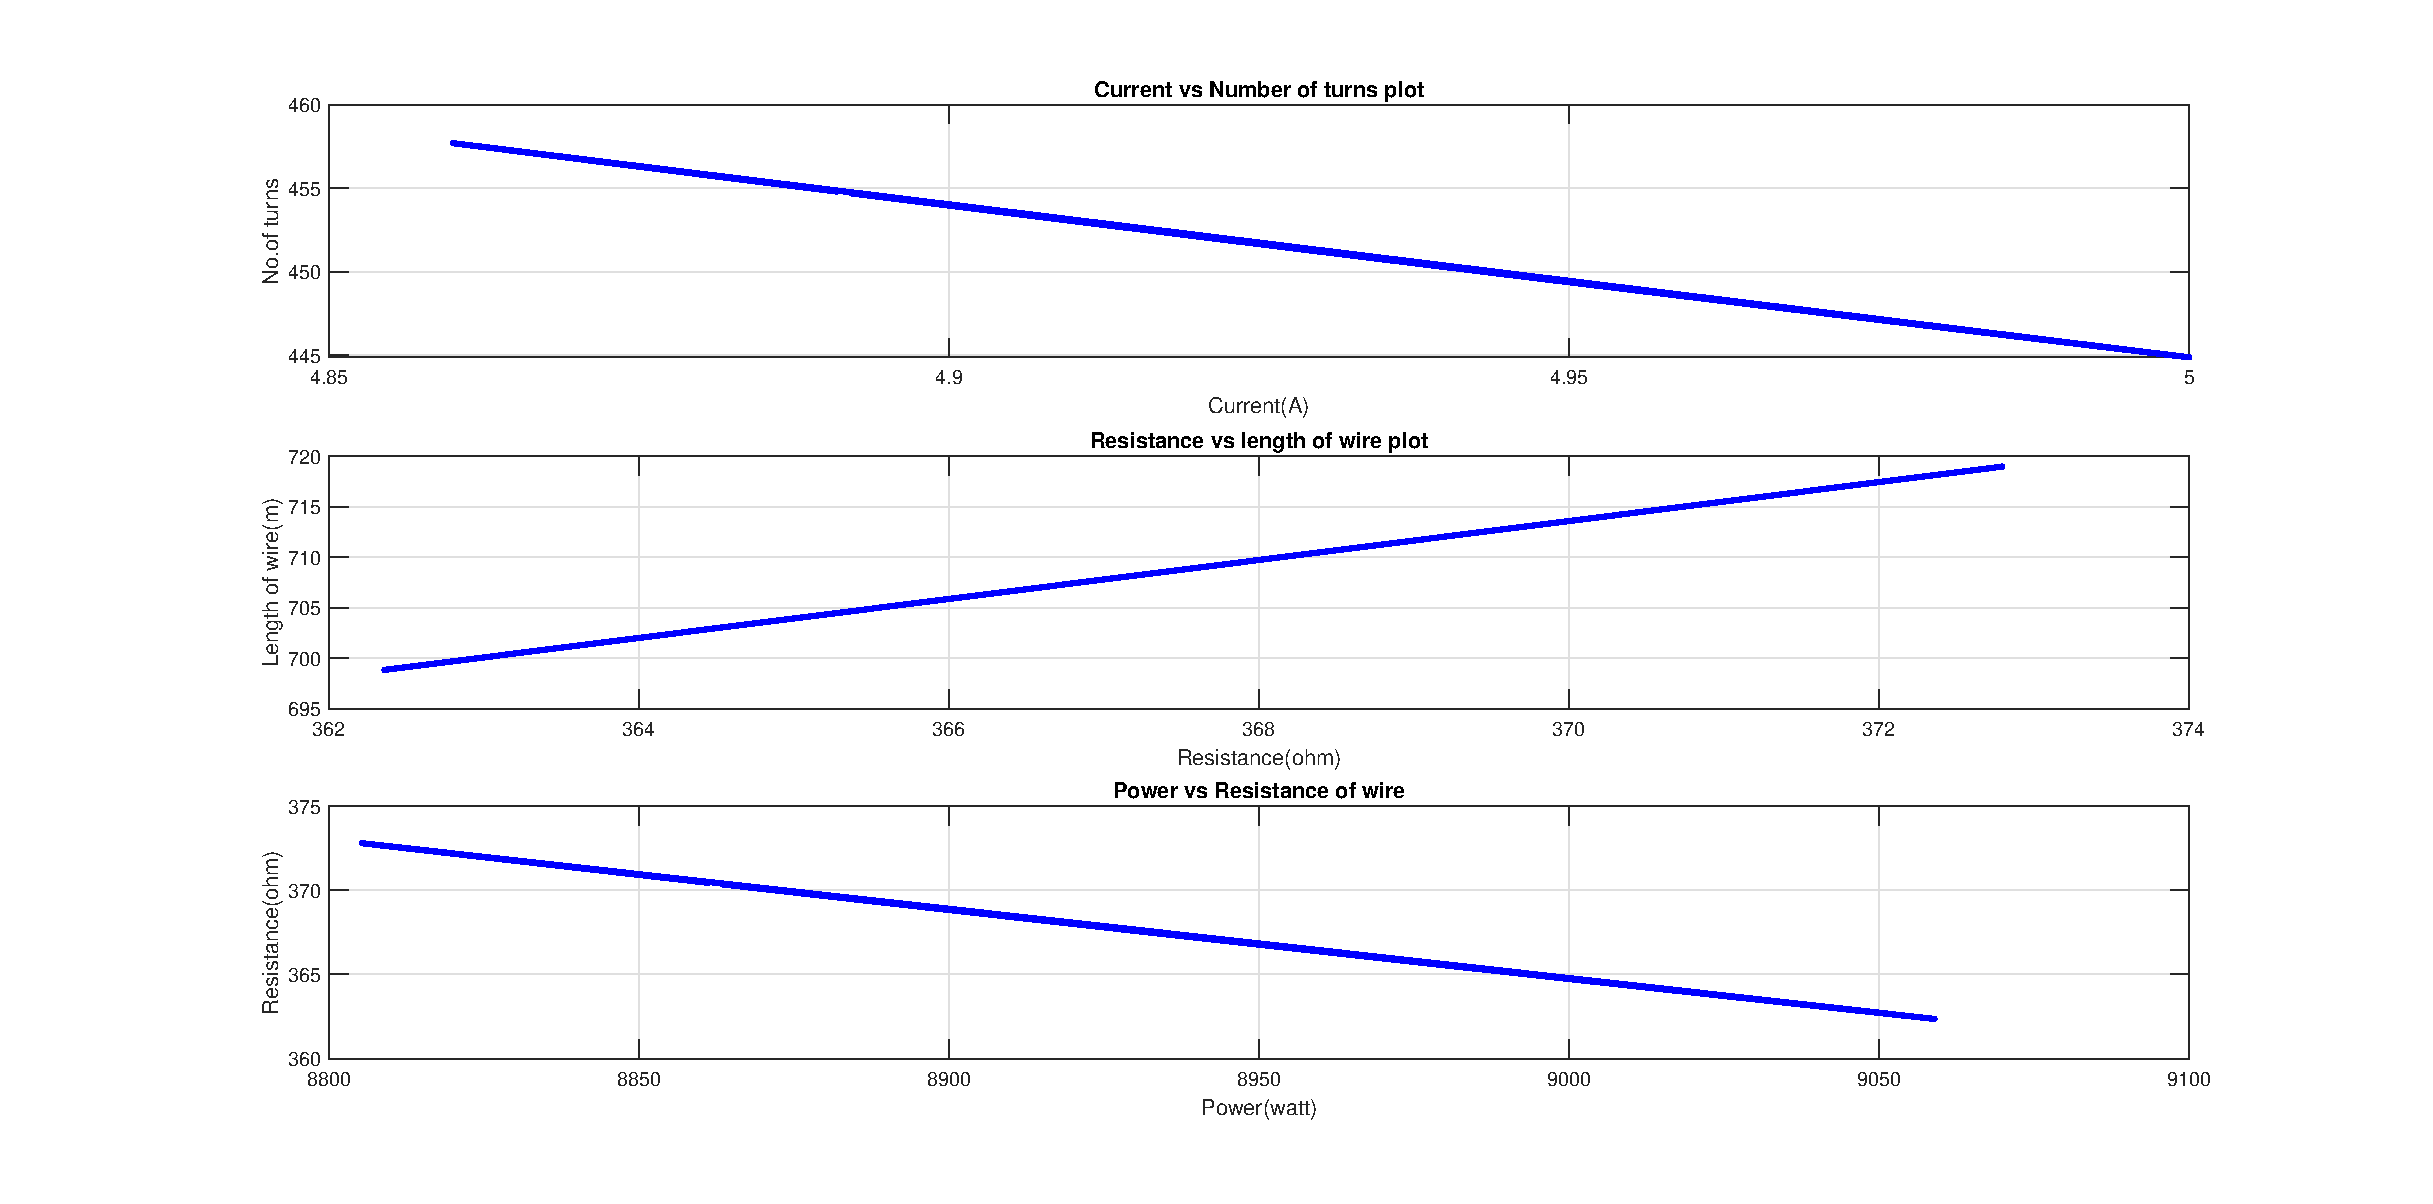
\includegraphics[width=4in,height=3in]{images/fix_guage.eps}
	\caption{Graphs used for fixing wire gauge}
	\label{fig-wVt}
\end{figure}

\subsection{Miniature model of Helmholtz coil}
To check our theoretical assumptions before the fabrication of actual helmholtz coil we made a miniature model by 3D printing it with ABS(Acrylonitrile Butadiene Styrene) with diameter 10cm and winded with 28 AWG copper wire.

\par We tested it and proved that the theoretical value of the magnetic field at the centre of the two coils is equal to the practical value of magnetic field measured using EMF detector.


\subsection{Fabrication of Helmholtz coil}

We wound the wire around the plywood frame ,150 turns per coil, which was calculated from the formula.The Helmholtz coil is designed to produce 3mT magnetic field and   current. Plywood was selected to build the framework of helmholtz coil. Plywood was choosed because of its relative permeability, which has the value close to that of air and also because it is easily available and is cheap. A hacksaw was used to to cut the plywood in the desired dimensions of the frame. In helmholtz coil distance between the centre of two coils should be equal to the radius of coil .A distance of 20cm was fixed taking into consideration of the desired  magnetic field produced ,since magnetic field is inversely proportional to distance and also considering the fact that the cubesat is 10 cm in width. Then we wound both the coils manually and a SMPS was used to control the voltage applied to the coil. Here we used a 12V SMPS according to our current requirement. We used a multimeter to measure the current flowing through the coil and measured the magnetic field using a mobile application.The magnetic field was found as 2.1mT. Thus we encountered an error of 8.6 percentage but it is neglible.The power draw was found out to be less than 60W.

\begin{figure}[h!]
	\centering
	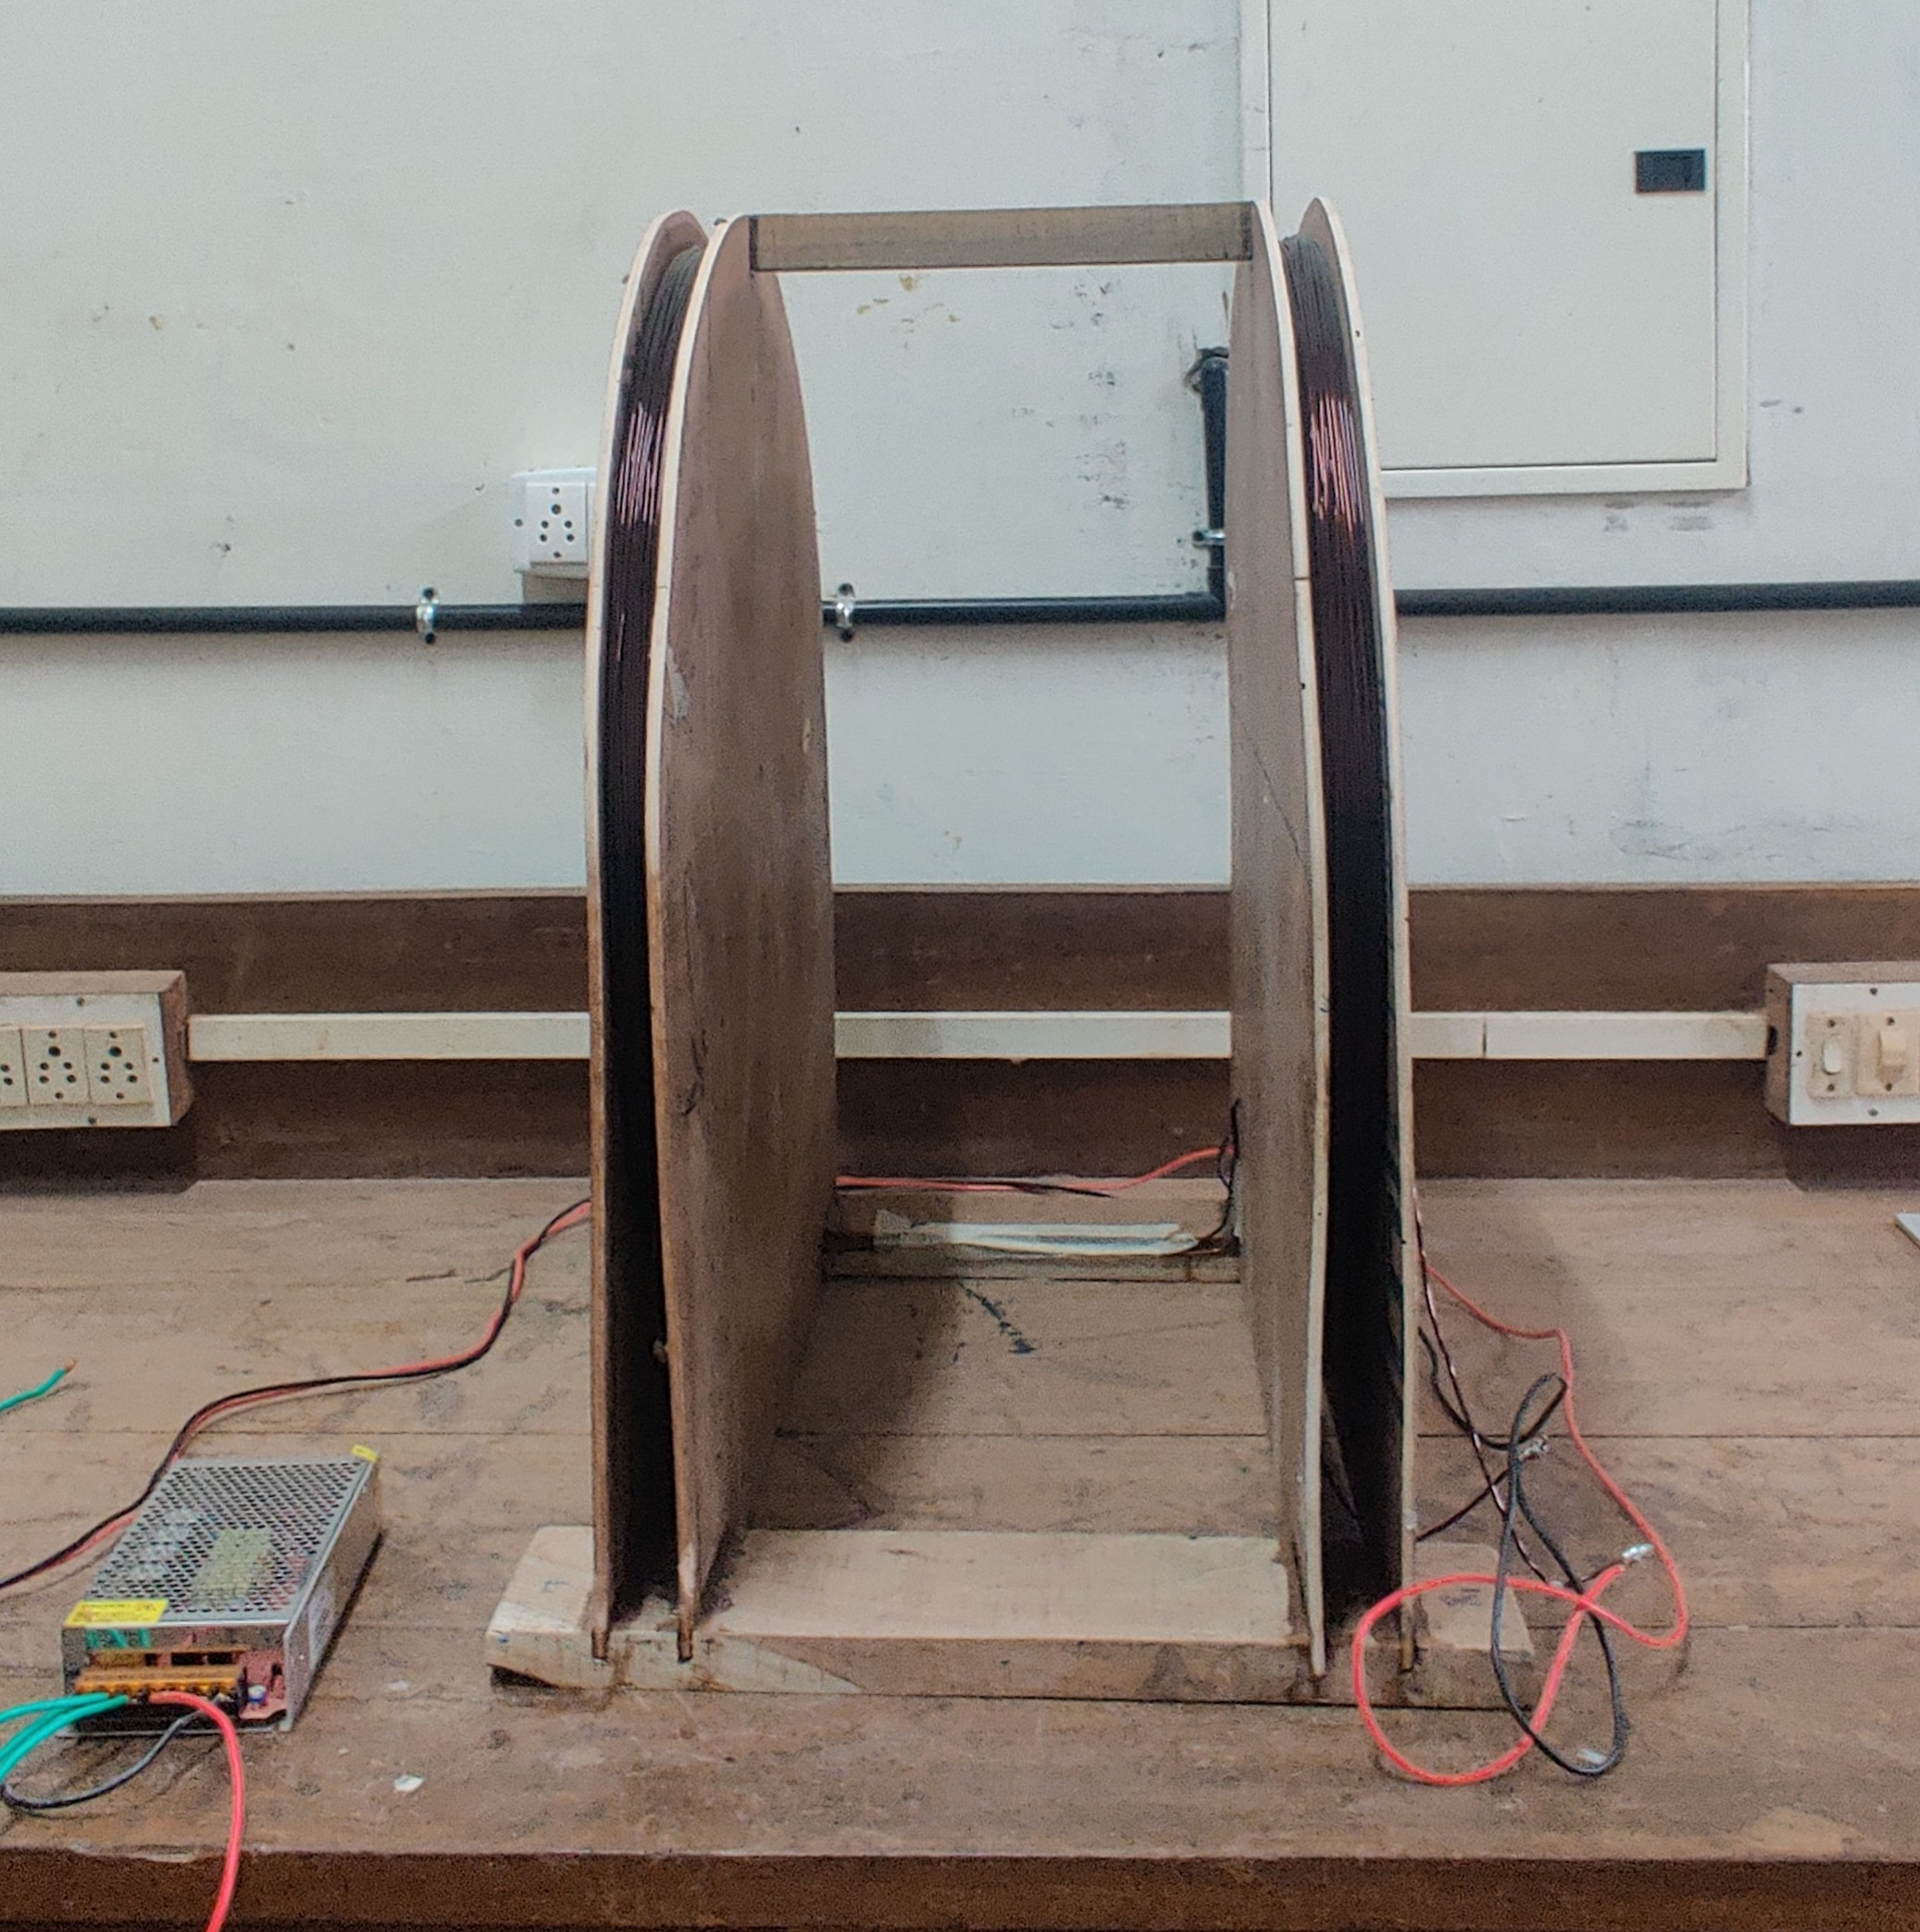
\includegraphics[width=3in,height=3in]{images/1pic.jpg}
	\caption{Helmholtz coil}
	\label{fig-wVt}
\end{figure}


\subsection{Result}

Desired uniform magnetic field is produced using the Helmholtz coil.
